\documentclass[12pt]{scrartcl}

 

\usepackage[utf8]{inputenc}

\usepackage[T1]{fontenc}

\usepackage{lmodern}

\usepackage[ngerman]{babel}

\usepackage{amsmath}

\usepackage{graphicx}


 

\title{Versuch E2\\ Der Halleffekt}

\author{Frederik Strothmann, Henrik Jürgens}

\date{\today}


\begin{document}


 %deckblatt erstellen

\maketitle
\tableofcontents
\newpage

%einleitung zu dem experiment

\section{Einleitung}

In diesem Versuch soll das Magnetfeld einer kurzen Spule auf ihrer Mittelachse ausmessen und dabei einfache elektrische Grundschaltungen angewendet werden. Zur Messung benutzen wir eine Hallsonde, die zu diesem Zweck vorher geeicht werden muß. Die Hallsonde liefert eine Spannung, die proportional zum Magnetfeld ist, aber schwierig zu messen ist, da sie im Millivoltbereich liegt und einige Hallsondentypen eine hohen Innenwiderstand haben. Die Ausgangsspannung der Hallsonde wird daher in diesem Versuch mit einer Kompensationsschaltung bestimmt. Den Widerstand der Hallsonde messen Sie mit der
Wheatstoneschen Brückenschaltung.

%versuchsaufbau mit skizze

\section{Versuchsaufbau}
Der Versuchsaufbau besteht haupsächlich aus zwei Komponenten, der Spule mit der Hallsonde und dem Steuerkasten.
Der Schaltplan ist in Abbilung \ref{fig:aufbau} zu sehen.

\begin{figure}[htbp] 
  \centering
    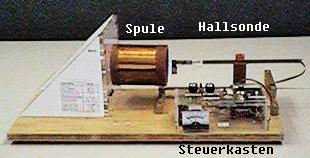
\includegraphics[scale = 0.5]{kasten_und_spule.JPG}
  	\caption[Foto der beiden Hauptbestandteile des Versuchs]{Foto der beiden Hauptbestandteile des Versuchs\footnotemark}
  \label{fig:kasten_und_spule}
\end{figure}
\footnotetext{Graphik wurde am 19.08.2014 von der Seite: http://www.atlas.uni-wuppertal.de/~kind/apjpg/ap1e2a.JPG entnommen}

\begin{figure}[htbp] 
  \centering
    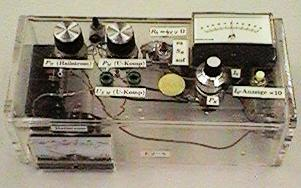
\includegraphics[scale = 0.5]{kasten.JPG}
  	\caption[Foto des Schaltkastens]{Foto des Schaltkastens\footnotemark}
  \label{fig:kasten}
\end{figure}
\footnotetext{Graphik wurde am 19.08.2014 von der Seite: http://www.atlas.uni-wuppertal.de/~kind/apjpg/ap1e2vkg.JPG entnommen}

\section{Versuchsdurchführung}


\subsection{Praktische Durchführung}

\begin{enumerate}
\item Schaltskizze \newline

\begin{figure}[htbp] 
	  \centering
	    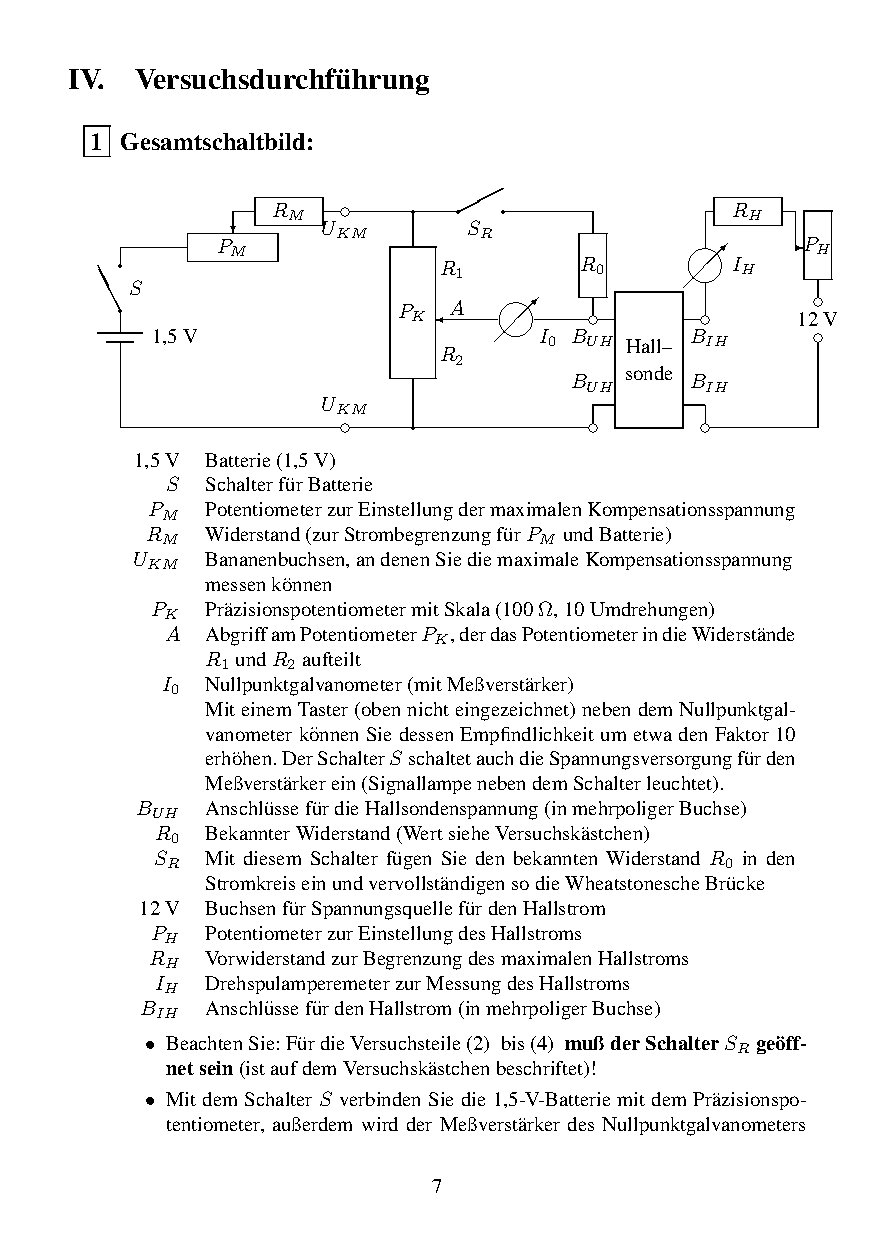
\includegraphics[trim = 1mm 135mm 1mm 30mm, clip, scale = 1]{aufbau.pdf}
	  	\caption[Schaltskizze des Versuchsaufbaus]{Schaltskizze des Versuchsaufbaus\footnotemark}
	  \label{fig:aufbau}
	\end{figure}
	\footnotetext{Abbildung entnommen von http://www.atlas.uni-wuppertal.de/~kind/E2.pdf Seite 7 am 19.08.2014}

\begin{itemize}
\item
1,5V: Batterie

\item
S: Schalter für die Batterie

\item
P$_\text{M}$: Potentiometer zum Einstellen der maximalen Kompensationsspannung

\item
R$_\text{M}$: Wiederstand für die Strombegrenzung von P$_\text{M}$ und der Batterie

\item
U$_\text{KM}$: Bananenbuchse, zum messen der Kompensationsspannung

\item
P$_\text{K}$: Präzisionspotentiometer mit Skala

\item
A: Abgriff am Potentiometer P$_\text{K}$, der das Potentiometer an die Widerstände R$_\text{1}$ und $_\text{2}$ aufteilt

\item
I$_\text{0}$: Nullpunktgalvanometer. Mit Taster zum erhöhen der Empfindlichkeit um den Faktor 10. S schaltet den Messverstärker ein.

\item
B$_\text{UH}$: Anschlüsse für die Hallsondenspannung

\item
R$_\text{0}$: Bekannter Widerstand

\item
S$_\text{R}$: Schalter um den Widerstand R$_\text{0}$ in den Stromkreis einzufügen und die Wheatstonesche Brücke zu vervollständigen

\item
12V: Buchsen für Spannungsquelle des Hallstroms

\item
P$_\text{H}$: Potentiometer zum einstellen des Hallstroms

\item
R$_\text{H}$: Vorwiderstand zur Begrenzung des Hallstroms

\item
I$_\text{H}$: Drehspulamperemeter zur Messung des maximalen Hallstroms

\item
B$_\text{IH}$: Anschlüsse für den Hallstrom

\end{itemize}

\item
Vorversuche: \newline
\begin{enumerate}
\item
Schließen Sie die Spule an das Netzgerät an und stellen Sie einen Strom von 1A ein. Achten Sie auf die richtige Polarität des Magnetfeldes, damit es keine negativen Hallspannungen gibt (siehe b)).
\newline
\item
Schließen Sie an die Buchsen mit der Bezeichnung 12 Volt für I-Hall des Versuchskästchens die 12–Volt–Festspannungsquelle an. Achten Sie auf die angegebene Polarität (+ und –). Die Hallsonde kann zwar mit beliebiger Stromrichtung arbeiten. In Ihrem Versuchskästchen befindet sich aber ein weiteres Drehspulamperemeter für den Hallstrom, das keine negativen Ströme anzeigen kann. Außerdem würden Sie negative Hallspannungen bekommen, die
Sie mit der gegebenen Schaltung nicht kompensieren können. Stellen Sie den
maximalen Hallstrom ein (Je nach
Sondentyp liegt der maximale Hallstrom zwischen 5 und 100 mA. Der Vorwiderstand
R$_H$ im Versuchskästchen begrenzt den Hallstrom auf zulässige Werte).
\newline
\item
Schieben Sie die Hallsonde in die Mitte der Spule. Stellen Sie dann eine maximale Kompensationsspannung so ein, daß bei dieser Anordnung die Hallspannung noch kompensiert werden kann und gleichzeitig eine leichte Umrechnung von Skalenteilen auf die Kompensationsspannung (zwischen Punkt A und dem unteren Punkt U$_{KM}$) möglich ist. Die Potentiometerskala zeigt Ihnen das Verhältnis von R$_2$ zu R$_1$ + R$_2$.
”0“ bedeutet R$_2$ = 0$\Omega$,”10“ (oder
0,00 hinter 9,99) bedeutet R$_1$ = 0$\Omega$. Da sich die Spannung der Batterie im Laufe der Zeit verändern kann, sollten Sie U$_{KM}$ öfter überprüfen und gegebenenfalls korrigieren
\end{enumerate}
\item
Eichung der Hallsonde 
\newline
\begin{enumerate}
\item
Bestimmen Sie den Ort der Hallsonde in der Spule, an dem die Hallspannung maximal ist. In diesem Punkt können Sie annehmen, daß eine unendlich lange
Spule vorliegt. (Schätzen Sie die Winkel
$\theta_1$ und $\theta_2$ aus 
\begin{align}
\text{B}_z = \frac{1}{2} \mu_0 \text{I}_S \text{N} (\cos(\theta_1) - \cos(\theta_2))
\label{eqn:Aufgabe 3_PD_B-Feld_1} 
\end{align}

\begin{figure}[htbp] 
	  \centering
	    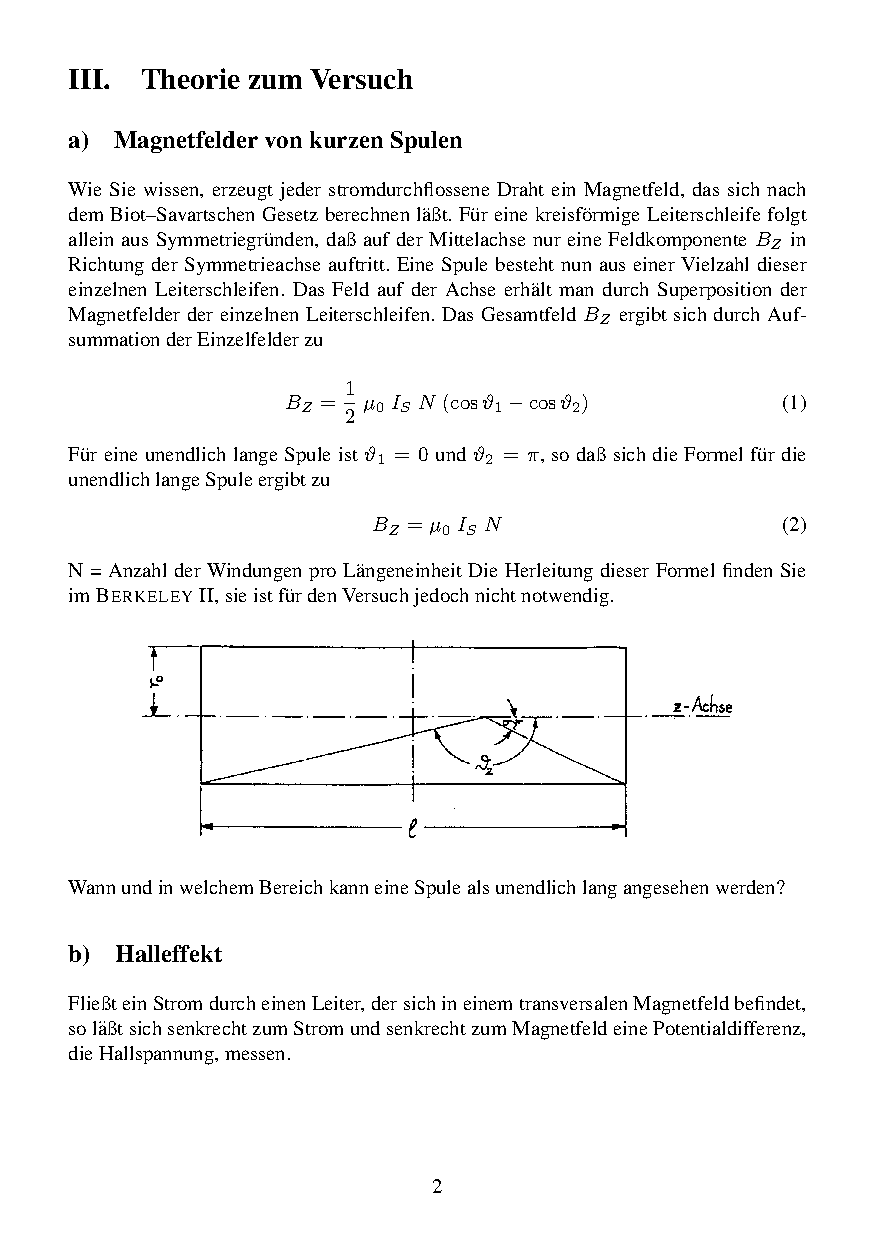
\includegraphics[trim = 1mm 62mm 1mm 105mm, clip, scale = 1]{winkel.pdf}
	  	\caption[Skizze der Winkel für das Biot-Savat-Gesetz in einer kurzen Spule]{Skizze der Winkel für das Biot-Savat-Gesetz in einer kurzen Spule\footnotemark}
	  \label{fig:winkel}
	\end{figure}
	\newpage
	\footnotetext{Abbildung entnommen von http://www.atlas.uni-wuppertal.de/~kind/E2.pdf Seite 2 am 19.08.2014}
	

 ab und vergleichen Sie den gemessenen Wert des Magnetfeldes mit dem Wert nach
 \begin{align}
 \text{B}_Z = \mu_0 \text{I}_S \text{N}
 \label{eqn:Aufgabe 3_PD_B-Feld_2}
\end{align}
 Für N können Sie einen Wert von 13000/m annehmen; die Spule hat 10 Lagen mit etwa 1300 Windungen pro Meter).
\newline
\item
Messen Sie dort die Abhängigkeit der Hallspannung vom Magnetfeld, indem
Sie den Spulenstrom variieren (0 bis 1 A) und das Magnetfeld nach Gleichung \ref{eqn:Aufgabe 3_PD_B-Feld_2} berechnen.
\newline
\item
Bestimmen Sie nun aus dieser Messung die Hallkonstante der Sonde, (die Sondendicke
d ist am Versuchsaufbau und in der Tabelle (letzte Seite) angegeben). Stellen Sie die Meßwerte graphisch dar. Beachten Sie, daß auch ohne Magnetfeld eine Hallspannung
U$_{HO}$ meßbar ist.

\begin{figure}[htbp] 
	  \centering
	    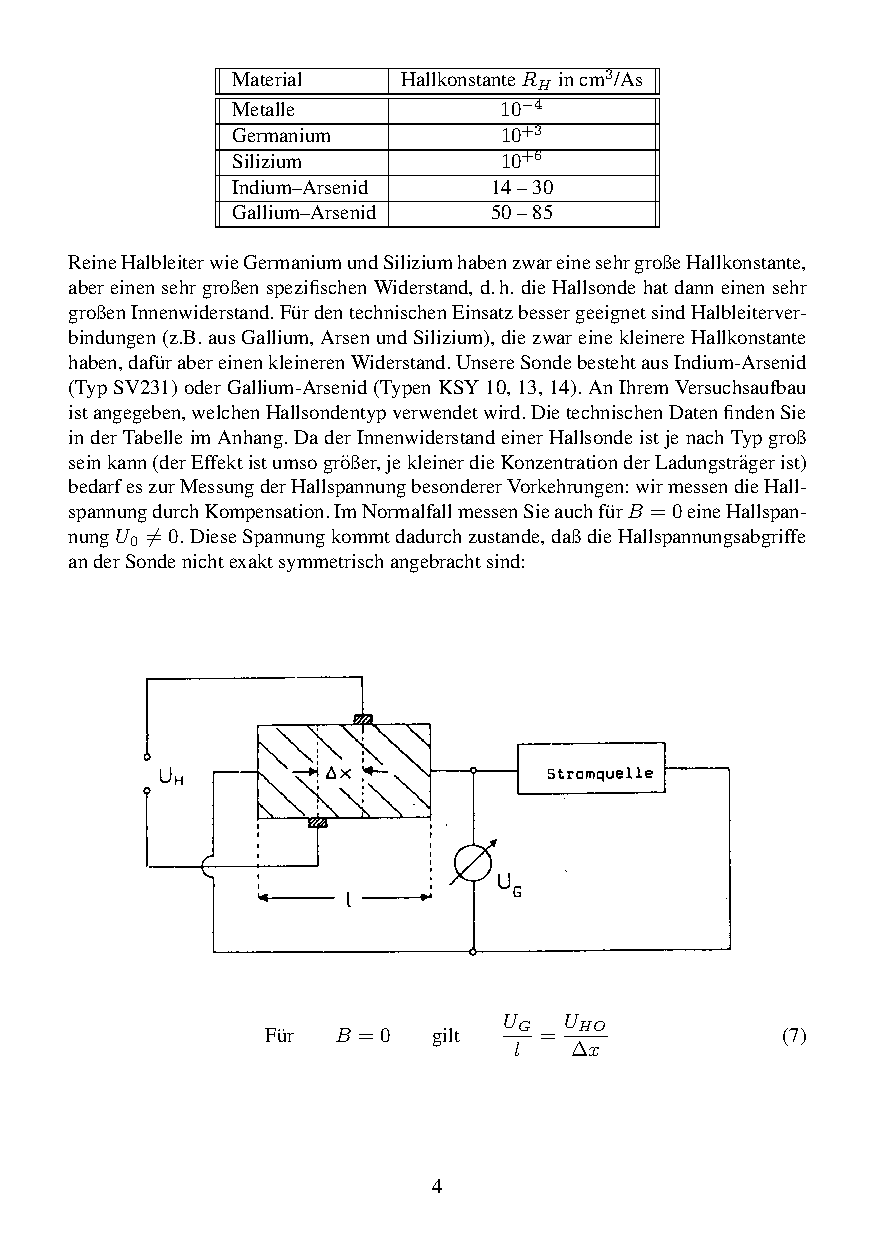
\includegraphics[trim = 1mm 40mm 1mm 105mm, clip, scale = 1]{U0H.pdf}
	  	\caption[Skizze für das abgreifen der Hallspannung wenn kein B-Feld vorhanden ist]{Skizze für das abgreifen der Hallspannung wenn kein B-Feld vorhanden ist\footnotemark}
	  \label{fig:U0H}
	\end{figure}
	\newpage
	\footnotetext{Abbildung entnommen von http://www.atlas.uni-wuppertal.de/~kind/E2.pdf Seite 4 am 19.08.2014}

\begin{align}
\frac{\text{U}_G}{\text{l}} = \frac{\text{U}_{HO}}{\Delta\text{x}}
\label{eqn: U_H0}
\end{align}
\newline
\item
Berechnen Sie aus der Hallkonstanten die Konzentration von freien Elektronen in Ihrem Sondenmaterial.
\newline
\item
Zeigen Sie, daß die Hallspannung linear vom Hallstrom abhängt. Messen Sie
jeden Punkt mit und ohne Magnetfeld (B = const.)
\end{enumerate}
\item
Messung des Magnetfeldes einer kurzen Spule 
\newline
\begin{enumerate}
\item
Stellen Sie wieder die Werte aus Versuch (2) ein und messen Sie das Feld der Spule auf der Symmetrieachse aus.
\newline
\item
Vergleichen Sie die Meßwerte an einigen Stellen mit dem Ergebnis aus Gleichung \ref{eqn:Aufgabe 3_PD_B-Feld_1}.
\end{enumerate}
\item
Messung des Widerstandes der Hallsonde \newline
\begin{enumerate}
\item
Bauen Sie eine Wheatstonesche Brückenschaltung mit Ihrer Meßapparatur
auf. Dazu schließen Sie den Schalter
S$_R$. Schalten Sie den Hallstrom aus (stöpseln Sie die Spannungsquelle für den Hallstrom ab)!

%bitte Schaltskizze einfügen
\begin{figure}[htbp] 
	\centering
		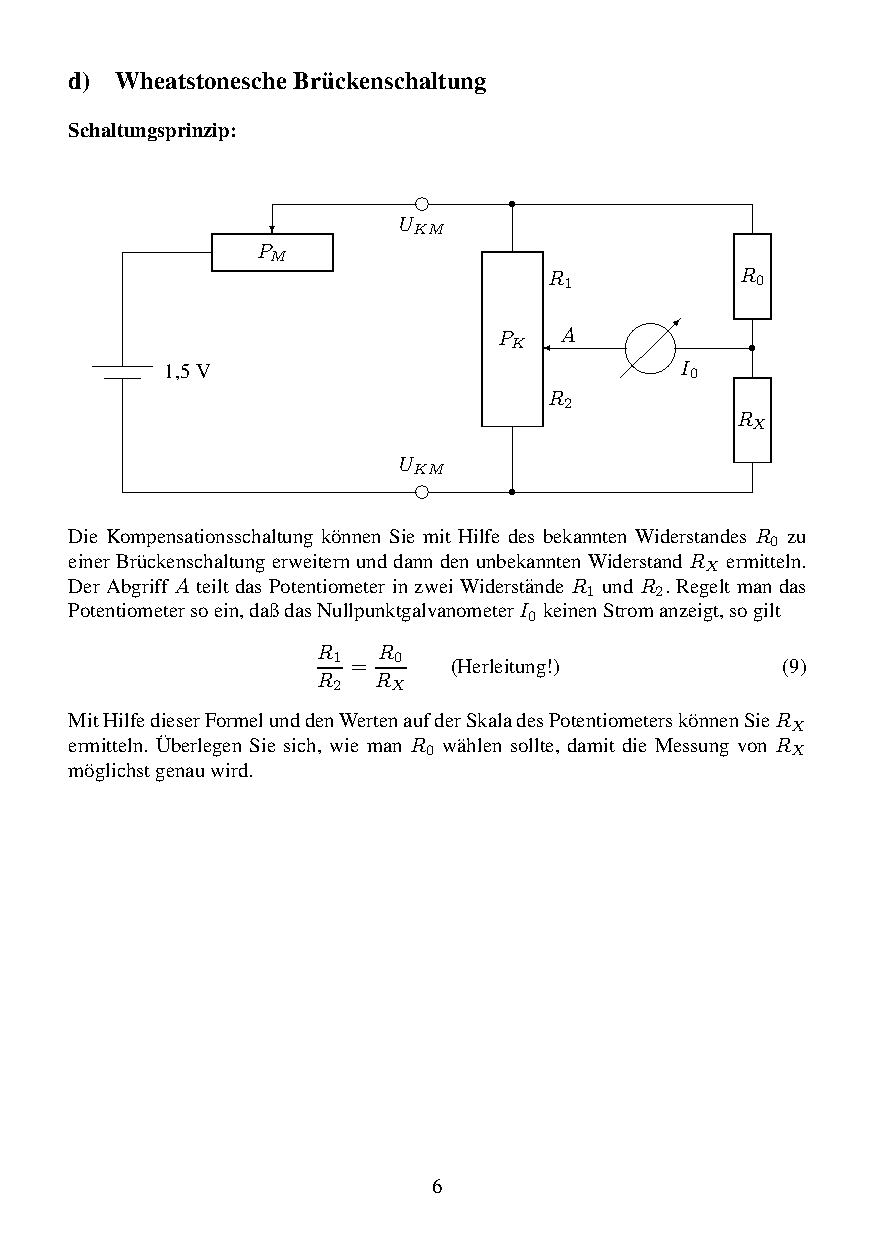
\includegraphics[trim = 1mm 125mm 1mm 30mm, clip, scale = 1]{wheat.pdf}
		\caption[Skizze Wheatstoneschen Brückenschaltung]{Skizze Wheatstoneschen Brückenschaltung\footnotemark}
		\label{fig:wheat}
\end{figure}

\footnotetext{Abbildung entnommen von http://www.atlas.uni-wuppertal.de/~kind/E2.pdf Seite 6 am 19.08.2014}


\item
Die Spannung U$_{KM}$ hat sich nun deutlich verringert (warum?).
Überlegen Sie sich, ob Sie das korrigieren und/oder in Ihrer Rechnung berücksichtigen
müssen.
\newline
\item
Bestimmen Sie nun den (Innen–)Widerstand Ihrer Hallsonde. Der Wert des bekannten Widerstandes R$_0$ ist auf dem Versuchskästchen angegeben.
\newline
\item
Sie können annehmen, daß der Widerstand, den die Hallsonde für den Hallstrom darstellt, etwa so groß wie der gerade bestimmte Innenwiderstand ist. Welche Spannung U$_G$ (siehe Gleichung \ref{eqn: U_H0}) fällt somit bei maximalem Hallstrom an der Sonde ab? Berechnen Sie aus der Spannung U$_{HO}$, die Sie bei maximalem Hallstrom gemessen haben, mit Hilfe von Gleichung \ref{eqn: U_H0} die Stecke $\Delta$x, um die die Hallspannungsabgriffe versetzt sind. Für die Länge der Hallsonde
l können Sie die Werte der Tabelle annehmen.
\end{enumerate}
\end{enumerate}

\subsection{Theoretische Durchführung}

\begin{enumerate}
\item[3.]
\begin{enumerate}
\item
Der Wert des Magnetfeldes berechnet sich durch:
\begin{align}
 \text{B}_Z = \mu_0 \text{I}_S \text{N}
 \label{eqn:Aufgabe 3_TD_B-Feld_2}
\end{align}
B die Magnetische Flussdichte auf der Z-Achse, I$_S$ der Spulenstrom und N die Windungszahl pro Längeneinheit.\\
mit einem Fehler von:
\begin{align}
\sigma_{\text{B}_Z} = \mu_0 \text{N} \sigma_{\text{I}_S}
\label{eqn:Aufgabe 3_TD_B-Feld_2_Fehler}
\end{align}
N wurde als Fehlerfrei angenommen.\\
\item
Folgender Zusammenhang ist zwischen Hallspannung und Magnetischer Flussdichte zu erwarten:
\begin{align}
\text{U}_H = \frac{1}{ne} \text{I}_H \text{B} \frac{1}{d}
\label{eqn:Hallspannung}
\end{align}
e die Elementarladung, n die Anzahl der Ladungen pro Volumenelement, I$_H$ der Hallstrom und B die Magnetische Flussdichte.\\
Die Hallspannung messen wir mithilfe einer Kompensationsschaltung nach folgender Formel:
\begin{align}
\text{U}_H = \text{U}_{KM} \frac{\text{R}_2}{\text{R}_1+\text{R}_2}
\label{eqn:U_H}
\end{align}
Mit dem Fehler:
\begin{align}
\sigma_{\text{U}_H} = \sqrt{
\left(\frac{\text{R}_2}{\text{R}_1+\text{R}_2}\sigma_{\text{U}_{KM}}\right)^2+
\left(\text{U}_{KM}\sigma_{\frac{\text{R}_2}{\text{R}_1+\text{R}_2}}\right)^2}
\label{eqn:U_H_Fehler}
\end{align}
Das Verhältnis R$_2$ zu R$_1$ + R$_2$ wird am Potentiometer abgelesen.\\
Die Magnetische Flussdichte wird nach Gleichung \ref{eqn:Aufgabe 3_TD_B-Feld_2} und dessen Fehler mit Gleichung \ref{eqn:Aufgabe 3_TD_B-Feld_2_Fehler} berechnet.
\item
Die Hallkonstante $\frac{1}{\text{ne}}$ berechnen wir nach Gleichung \ref{eqn:Hallspannung}:
\begin{align}
\frac{1}{ne} = \frac{\text{m} \text{d}}
{\text{I}_H}
\label{eqn:hallkonstante}
\end{align}
m ist die Steigung der Geraden die sich aus dem Plot von U$_H$ gegen B ergibt.\\
Mit einem Fehler von:
\begin{align}
\sigma_{\frac{1}{\text{ne}}} = 
\sqrt{\left(\frac{\text{d}}
{\text{I}_H}\sigma_{\text{m}}\right)^2+
\left(\frac{m}
{\text{I}_H}\sigma_{\text{d}}\right)^2+
\left(\frac{\text{m} \text{d}}
{\text{I}_H^2}\sigma_{\text{I}_H}\right)^2}
\label{eqn:Hallspannung_Fehler}
\end{align}
\item
Die Konzentration an freien Elektronen Berechnet sich durch:
\begin{align}
\text{n} = \frac{1}{\text{e}\frac{1}{\text{ne}}}
\label{eqn:freie_elektronen}
\end{align}
Mit einem Fehler von:
\begin{align}
\sigma_n = \frac{1}{\text{e}\left(\frac{1}{\text{ne}}\right)^2}\sigma_{\frac{1}{\text{ne}}}
\label{eqn:freie_elektronen_sigma}
\end{align}
e wird als fehlerlos betrachtet.
\item
Zu erwarten ist die Abhängigkeit von Hallspannung zu Hallstrom nach Gleichung \ref{eqn:Hallspannung}
\end{enumerate}
\item[4.]
\begin{enumerate}
\item
Das B-Feld wird nach Gleichung \ref{eqn:Hallspannung} bestimmt:
\begin{align*}
 \text{B}= \frac{\text{U}_H \text{d}}{\frac{1}{ne} \text{I}_H}
\end{align*}
mit einem Fehler von:
\begin{align}
\sigma_{\text{B}} = 
\sqrt{\left(\frac{\text{d}}
{\text{I}_H \frac{1}{\text{ne}}}\sigma_{\text{U}_H}\right)^2+
\left(\frac{\text{U}_H}
{\text{I}_H \frac{1}{\text{ne}}}\sigma_{\text{d}}\right)^2+
\left(\frac{\text{U}_H \text{d}}
{\text{I}_H^2 \frac{1}{\text{ne}}}\sigma_{\text{I}_H}\right)^2+
\left(\frac{\text{U}_H \text{d}}
{\text{I}_H \frac{1}{\text{ne}}^2}\sigma_{\frac{1}{\text{ne}}}\right)^2}
\end{align}
U$_H$ wird wieder mit Gleichung \ref{eqn:U_H}
und zugehörigem Fehler ermittelt.
\item
Die Messerte für das B-Feld sollen mit der Formel
\begin{align}
\text{B}_z = \frac{1}{2} \mu_0 \text{I}_S \text{N} (\cos(\theta_1) - \cos(\theta_2))
\label{eqn:Aufgabe 3_TD_B-Feld_1} 
\end{align}
verglichen werden.\\
Der zugehörige Fehler für die Vergleichswerte ist:
\begin{align}
\sigma_{\text{B}_z} = \frac{1}{2} \mu_0 \text{N}
\sqrt{\left((\cos(\theta_1) - \cos(\theta_2)) \sigma_{\text{I}_S}\right)^2+
\left(\text{I}_S \sin(\theta_1) \sigma_{\theta_1}\right)^2+
\left(\text{I}_S \sin(\theta_2) \sigma_{\theta_2}\right)^2}
\label{eqn:aufgabe_3_sigma}
\end{align}
\end{enumerate}
\item[5.]
\begin{enumerate}
\item[c)] Der Innenwiderstand der Hallsonde lässt sich nach folgender Formel berechnen:
\begin{align}
\text{R}_X = \frac{\text{R}_0}{1-\frac{\text{R}_2}{\text{R}_1+\text{R}_2}}\frac{\text{R}_2}{\text{R}_1+\text{R}_2}
\label{eqn:innen_widerstand}
\end{align}
Mit dem Fehler:
\begin{align}
\sigma_{\text{R}_X} = \sqrt{\left(\frac{\text{R}_0}{\left(\frac{1}{\frac{\text{R}_2}{\text{R}_1+\text{R}_2}}-1\right)^2}\frac{1}{\left(\frac{\text{R}_2}{\text{R}_1+
\text{R}_2}\right)^2}\sigma_{\frac{\text{R}_2}{\text{R}_1+\text{R}_2}}\right)^2}
\label{eqn:innen_widerstand_sigma}
\end{align}

\item[d)]
Die Formel für die Berechnung der Strecke $\Delta$x ist:
\begin{align}
\Delta \text{x} = \frac{\text{U}_{H0}\text{l}}{\text{U}_G}
\label{eqn:delta}
\end{align}
Mit einem Fehler von:
\begin{align}
\sigma_{\Delta \text{x}} = \sqrt{
\left(\frac{\text{l}}{\text{U}_G}\sigma_{\text{U}_{H0}}\right)^2+
\left(\frac{\text{U}_{H0}}{\text{U}_G}\sigma_{\text{l}}\right)^2+
\left(\frac{\text{U}_{H0}\text{l}}{\text{U}_G^2}\sigma_{\text{U}_G}\right)^2}
\label{eqn:delta_sigma}
\end{align}
\end{enumerate}

\end{enumerate}

\section{Messergebnisse}


\section{Messergebnisse}

\subsection{Aufgabe 3}
\begin{table}[htbp]
\caption{Messwerte für Aufgabe 3 a)}
\begin{center}
\begin{tabular}{|l|l|l|l|}
\hline
N & I\_S[A] & Fehler & myh\_null \\ \hline
\multicolumn{1}{|r|}{13000} & \multicolumn{1}{r|}{1} & \multicolumn{1}{r|}{0,01} & \multicolumn{1}{r|}{1,2566370614E-006} \\ \hline
d\_Spule[m] & Fehler & l\_Spule[m] & Fehler \\ \hline
\multicolumn{1}{|r|}{0,1033} & \multicolumn{1}{r|}{0,001} & \multicolumn{1}{r|}{0,1026} & \multicolumn{1}{r|}{0,001} \\ \hline
Theta\_1 & Fehler & Theta\_2 & Fehler \\ \hline
\multicolumn{1}{|r|}{45,1947882037} & \multicolumn{1}{r|}{0,0096442238} & \multicolumn{1}{r|}{134,8052117963} & \multicolumn{1}{r|}{0,0096442238} \\ \hline
\end{tabular}
\end{center}
\label{aufgabe_3_a}
\end{table}

\begin{table}[htbp]
\caption{Messwerte für Aufgabe 3 b)}
\begin{center}
\begin{tabular}{|r|r|r|r|r|r|r|r|}
\hline
\multicolumn{1}{|l|}{I\_S[A]} & \multicolumn{1}{l|}{Fehler} & \multicolumn{1}{l|}{U\_KM[V]} & \multicolumn{1}{l|}{Fehler} & \multicolumn{1}{l|}{R\_2/(R\_1+ R\_2)} & \multicolumn{1}{l|}{Fehler} & \multicolumn{1}{l|}{U\_H[V]} & \multicolumn{1}{l|}{Fehler} \\ \hline
1 & 0,01 & 0,1 & 0,006 & 0,364 & 0,02 & 0,036 & 0,003 \\ \hline
0,9 & 0,01 & 0,1 & 0,006 & 0,378 & 0,02 & 0,038 & 0,003 \\ \hline
0,8 & 0,01 & 0,1 & 0,006 & 0,398 & 0,02 & 0,040 & 0,003 \\ \hline
0,7 & 0,01 & 0,1 & 0,006 & 0,416 & 0,02 & 0,041 & 0,003 \\ \hline
0,6 & 0,01 & 0,1 & 0,006 & 0,432 & 0,02 & 0,043 & 0,003 \\ \hline
0,5 & 0,01 & 0,1 & 0,006 & 0,452 & 0,02 & 0,045 & 0,003 \\ \hline
0,4 & 0,01 & 0,1 & 0,006 & 0,47 & 0,02 & 0,047 & 0,003 \\ \hline
0,3 & 0,01 & 0,1 & 0,006 & 0,486 & 0,02 & 0,049 & 0,004 \\ \hline
0,2 & 0,01 & 0,1 & 0,006 & 0,506 & 0,02 & 0,051 & 0,004 \\ \hline
0,1 & 0,01 & 0,1 & 0,006 & 0,52 & 0,02 & 0,052 & 0,004 \\ \hline
0 & 0,01 & 0,1 & 0,006 & 0,538 & 0,02 & 0,054 & 0,004 \\ \hline
\end{tabular}
\end{center}
\label{aufgabe_3_b}
\end{table}


\begin{table}[htbp]
\caption{Messwerte für Aufgabe 3 c)}
\begin{center}
\begin{tabular}{|l|l|}
\hline
d\_sonde[myko meter] & Fehler \\ \hline
\multicolumn{1}{|r|}{0,0000025} & \multicolumn{1}{r|}{0,5} \\ \hline
I\_H[A] & Fehler \\ \hline
\multicolumn{1}{|r|}{0,1} & \multicolumn{1}{r|}{0,005} \\ \hline
U\_H/B & Fehler \\ \hline
\multicolumn{1}{|r|}{-1,07958} & \multicolumn{1}{r|}{0,008779} \\ \hline
e & Fehler \\ \hline
\multicolumn{1}{|r|}{1,602176565E-019} & \multicolumn{1}{r|}{0,000000022} \\ \hline
\end{tabular}
\end{center}
\label{aufgabe_3_c}
\end{table}


\begin{table}[htbp]
\caption{Messwerte für Aufgabe 3 e) mit Magnetfeld}
\begin{center}
\begin{tabular}{|r|r|r|r|r|r|r|r|}
\hline
\multicolumn{1}{|l|}{U\_KM[V]} & \multicolumn{1}{l|}{Fehler} & \multicolumn{1}{l|}{R\_2/(R\_1+ R\_2)} & \multicolumn{1}{l|}{Fehler} & \multicolumn{1}{l|}{I\_H[A]} & \multicolumn{1}{l|}{Fehler} & \multicolumn{1}{l|}{U\_H[V]} & \multicolumn{1}{l|}{Fehler} \\ \hline
0,1 & 0,006 & 0,364 & 0,02 & 1 & 0,005 & 0,036 & 0,003 \\ \hline
0,1 & 0,006 & 0,32 & 0,02 & 0,9 & 0,005 & 0,032 & 0,003 \\ \hline
0,1 & 0,006 & 0,282 & 0,02 & 0,8 & 0,005 & 0,028 & 0,003 \\ \hline
0,1 & 0,006 & 0,246 & 0,02 & 0,7 & 0,005 & 0,025 & 0,002 \\ \hline
0,1 & 0,006 & 0,222 & 0,02 & 0,6 & 0,005 & 0,022 & 0,002 \\ \hline
0,1 & 0,006 & 0,17 & 0,02 & 0,5 & 0,005 & 0,017 & 0,002 \\ \hline
0,1 & 0,006 & 0,134 & 0,02 & 0,4 & 0,005 & 0,013 & 0,002 \\ \hline
0,1 & 0,006 & 0,094 & 0,02 & 0,3 & 0,005 & 0,009 & 0,002 \\ \hline
0,1 & 0,006 & 0,068 & 0,02 & 0,2 & 0,005 & 0,007 & 0,002 \\ \hline
0,1 & 0,006 & 0,001 & 0,02 & 0 & 0,005 & 0,0001 & 0,002 \\ \hline
\end{tabular}
\end{center}
\label{aufgabe_3_e_m}
\end{table}

\begin{table}[htbp]
\caption{Messwerte für Aufgabe 3 e) ohne Magnetfeld}
\begin{center}
\begin{tabular}{|r|r|r|r|r|r|r|r|}
\hline
\multicolumn{1}{|l|}{U\_KM[V]} & \multicolumn{1}{l|}{Fehler} & \multicolumn{1}{l|}{R\_2/(R\_1+ R\_2)} & \multicolumn{1}{l|}{Fehler} & \multicolumn{1}{l|}{I\_H[A]} & \multicolumn{1}{l|}{Fehler} & \multicolumn{1}{l|}{U\_H[V]} & \multicolumn{1}{l|}{Fehler} \\ \hline
0,1 & 0,006 & 0,54 & 0,02 & 1 & 0,005 & 0,054 & 0,004 \\ \hline
0,1 & 0,006 & 0,482 & 0,02 & 0,9 & 0,005 & 0,048 & 0,004 \\ \hline
0,1 & 0,006 & 0,43 & 0,02 & 0,8 & 0,005 & 0,043 & 0,003 \\ \hline
0,1 & 0,006 & 0,376 & 0,02 & 0,7 & 0,005 & 0,038 & 0,003 \\ \hline
0,1 & 0,006 & 0,342 & 0,02 & 0,6 & 0,005 & 0,034 & 0,003 \\ \hline
0,1 & 0,006 & 0,266 & 0,02 & 0,5 & 0,005 & 0,027 & 0,003 \\ \hline
0,1 & 0,006 & 0,206 & 0,02 & 0,4 & 0,005 & 0,021 & 0,002 \\ \hline
0,1 & 0,006 & 0,152 & 0,02 & 0,3 & 0,005 & 0,015 & 0,002 \\ \hline
0,1 & 0,006 & 0,102 & 0,02 & 0,2 & 0,005 & 0,010 & 0,002 \\ \hline
0,1 & 0,006 & 0,001 & 0,02 & 0 & 0,005 & 0,0001 & 0,002 \\ \hline
\end{tabular}
\end{center}
\label{aufgabe_3_e_o}
\end{table}

\newpage

\subsection{Aufgabe 4}

\begin{table}[htbp]
\caption{Messwerte für Aufgabe 4}
\begin{center}
\begin{tabular}{|r|r|r|r|r|r|}
\hline
\multicolumn{1}{|l|}{I\_S[A]} & \multicolumn{1}{l|}{Fehler} & \multicolumn{1}{l|}{U\_KM[V]} & \multicolumn{1}{l|}{Fehler} & \multicolumn{1}{l|}{I\_H[A]} & \multicolumn{1}{l|}{Fehler} \\ \hline
1 & 0,005 & 0,1 & 0,006 & 0,1 & 0,005 \\ \hline
\multicolumn{1}{|l|}{Position [m]} & \multicolumn{1}{l|}{Fehler} & \multicolumn{1}{l|}{R\_2/(R\_1+ R\_2)} & \multicolumn{1}{l|}{Fehler} & \multicolumn{1}{l|}{U\_H[V]} & \multicolumn{1}{l|}{Fehler} \\ \hline
0,17 & 0,01 & 0,498 & 0,02 & 0,050 & 0,004 \\ \hline
0,16 & 0,01 & 0,484 & 0,02 & 0,048 & 0,004 \\ \hline
0,15 & 0,01 & 0,466 & 0,02 & 0,047 & 0,003 \\ \hline
0,14 & 0,01 & 0,448 & 0,02 & 0,045 & 0,003 \\ \hline
0,13 & 0,01 & 0,422 & 0,02 & 0,042 & 0,003 \\ \hline
0,12 & 0,01 & 0,402 & 0,02 & 0,040 & 0,003 \\ \hline
0,11 & 0,01 & 0,386 & 0,02 & 0,039 & 0,003 \\ \hline
0,1 & 0,01 & 0,374 & 0,02 & 0,037 & 0,003 \\ \hline
0,09 & 0,01 & 0,368 & 0,02 & 0,038 & 0,003 \\ \hline
0,08 & 0,01 & 0,368 & 0,02 & 0,038 & 0,003 \\ \hline
0,07 & 0,01 & 0,376 & 0,02 & 0,038 & 0,003 \\ \hline
0,06 & 0,01 & 0,384 & 0,02 & 0,038 & 0,003 \\ \hline
0,05 & 0,01 & 0,4 & 0,02 & 0,04 & 0,003 \\ \hline
0,04 & 0,01 & 0,42 & 0,02 & 0,042 & 0,003 \\ \hline
0,03 & 0,01 & 0,446 & 0,02 & 0,045 & 0,003 \\ \hline
0,02 & 0,01 & 0,466 & 0,02 & 0,047 & 0,003\\ \hline
\end{tabular}
\end{center}
\label{aufgabe_4}
\end{table}

\newpage

\subsection{Aufgabe 5}

\begin{table}[htbp]
\caption{Messwerte für Aufgabe 5}
\begin{center}
\begin{tabular}{|l|l|}
\hline
R\_0[Ohm] & Fehler \\ \hline
\multicolumn{1}{|r|}{49,9} & \multicolumn{1}{r|}{0,5} \\ \hline
R\_2(R\_1+R\_2) & Fehler \\ \hline
\multicolumn{1}{|r|}{0,364} & \multicolumn{1}{r|}{0,002} \\ \hline
R\_H[Ohm] & Fehler \\ \hline
\multicolumn{1}{|r|}{28,6} & \multicolumn{1}{r|}{0,4} \\ \hline
U\_KM[V] & Fehler \\ \hline
\multicolumn{1}{|r|}{0,46} & \multicolumn{1}{r|}{0,06} \\ \hline
I\_H[A] & Fehler \\ \hline
\multicolumn{1}{|r|}{0,1} & \multicolumn{1}{r|}{0,005} \\ \hline
U\_G[V] & Fehler \\ \hline
\multicolumn{1}{|r|}{2,9} & \multicolumn{1}{r|}{0,1} \\ \hline
l\_Spule[m] & Fehler \\ \hline
\multicolumn{1}{|r|}{0,1026} & \multicolumn{1}{r|}{0,001} \\ \hline
\end{tabular}
\end{center}
\label{aufgabe_5}

\section{Auswertung}

\subsection{Aufgabe 3}
In der ersten Teilaufgabe sollte das B-Feld auf zwei unterschiedliche Methoden bestimmt werden.
Der gemessene Wert nach Formel \ref{eqn:Aufgabe 3_PD_B-Feld_2} und der Fehler nach Formel \ref{eqn:Aufgabe 3_TD_B-Feld_2_Fehler} ergab 0,01633 $(\pm 0,0002)$ Tesla. Nach Formel \ref{eqn:Aufgabe 3_PD_B-Feld_1} und der Fehlerformel \ref{eqn:aufgabe_3_sigma} ergab sich ein Wert von 0,01151 $(\pm 0,0002)$ Tesla.

Im zweiten Aufgabenteil sollte die Abhängigkeit der Hallspannung vom Magnetfeld ermittelt werden. Dabei ergab sich der folgende Plot.

\begin{figure}[htbp] 
  \centering
    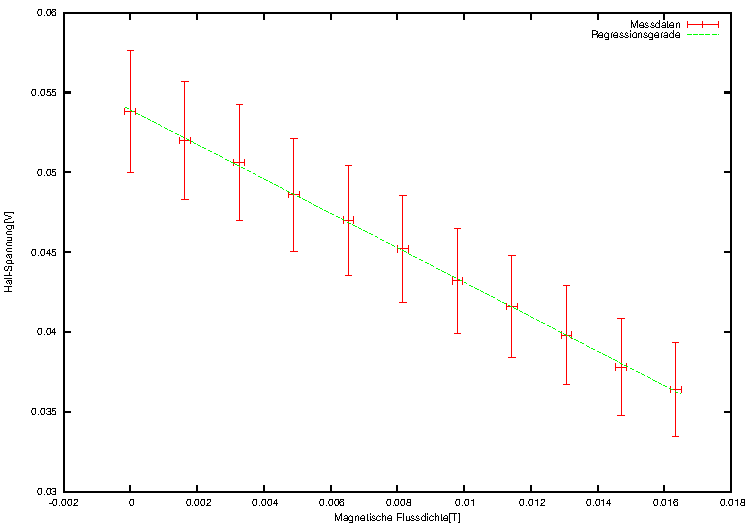
\includegraphics[scale = 1.3]{aufgabe_3_b.pdf}
  	\caption[Plot der Hallspannung in Abhängigkeit des Magnetfeldes]{Plot der Hallspannung in Abhängigkeit des Magnetfeldes}
  \label{fig:hall_mag}
\end{figure}

Im der dritten Teilaufgabe sollte die Hallkonstante mit Formel \ref{eqn:Hallspannung_Fehler} und der Fehler mit Formel \ref{eqn:Hallspannung_Fehler} bestimmt werden, wobei sich ein Wert von -2,70E-005 $(\pm 0,05E-005)$ m$^3$/C ergab.

Nun sollte n bestimmt werden, dafür wurde Formel \ref{eqn:freie_elektronen} und für den Fehler Formel \ref{eqn:freie_elektronen_sigma} verwendet. Es ergab sich ein Wert von -2,313E023 $(\pm 6,2277E015)$ Teilchen/m$^3$.

Im letzten Aufgabenteil sollte der Zusammenhang zwischen Hallspannung und Hallstrom ermittelt werden. Dafür wurde bei variierendem Hallstrom jeweils mit und ohne Magnetfeld gemessen.
Graphisch ergeben sich folgende lineare Plots:

\begin{figure}[htbp] 
  \centering
    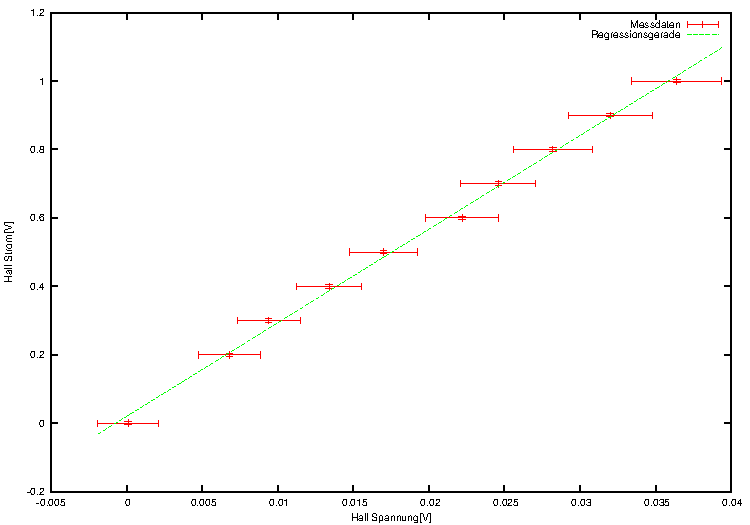
\includegraphics[scale = 1.3]{aufgabe_3_e_m.pdf}
  	\caption[Zusammenhang von Hallspannung und Hallstrom mit Magnetfeld]{Zusammenhang von Hallspannung und Hallstrom mit Magnetfeld}
  \label{fig:kasten}
\end{figure}

\begin{figure}[htbp] 
  \centering
    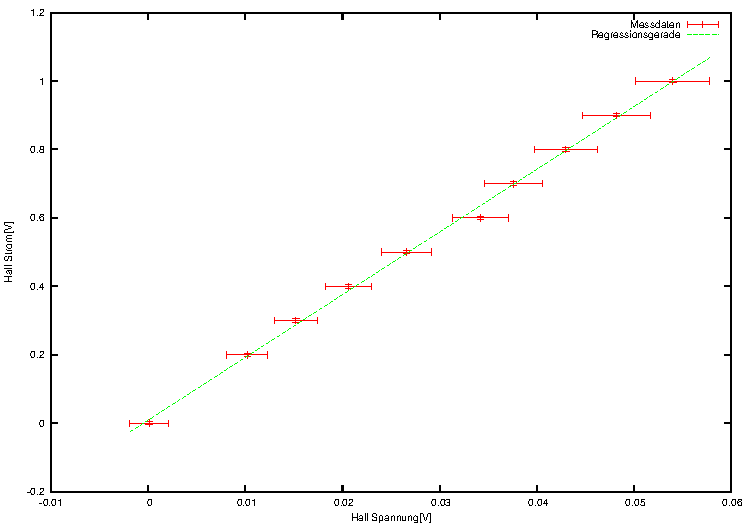
\includegraphics[scale = 1.3]{aufgabe_3_e_o.pdf}
  	\caption[Zusammenhang von Hallspannung und Hallstrom ohne Magnetfeld]{Zusammenhang von Hallspannung und Hallstrom ohne Magnetfeld}
  \label{fig:kasten}
\end{figure}

\newpage

\subsection{Aufgabe 4}
In Aufgabe 4 sollte das Magnetfeld auf der x-Achse ausgemessen werden und mit Werten, die mit Gleichung \ref{eqn:Aufgabe 3_PD_B-Feld_2} berechnet wurden, verglichen werden.

\begin{table}[htbp]
\caption{Vergleich der gemessenen Werte mit den aus den Materialeigenschaften bestimmten Werten.}
\begin{center}
\begin{tabular}{|r|r|r|r|}
\hline
\multicolumn{1}{|l|}{B-Feld[T]} & Fehler & \multicolumn{1}{l|}{B-Feld Formel [T]} & \multicolumn{1}{l|}{Fehler} \\ \hline
-0,0538 & 0,0005 & 0,014 & 0,008 \\ \hline
-0,0522 & 0,0005 & 0,013 & 0,009 \\ \hline
-0,0503 & 0,0005 & 0,013 & 0,011 \\ \hline
-0,0484 & 0,0005 & 0,012 & 0,013 \\ \hline
-0,0456 & 0,0005 & 0,011 & 0,016 \\ \hline
-0,0434 & 0,0004 & 0,010 & 0,020 \\ \hline
-0,0417 & 0,0004 & 0,008 & 0,026 \\ \hline
-0,0404 & 0,0004 & 0,006 & 0,036 \\ \hline
-0,0397 & 0,0004 & 0,003 & 0,057 \\ \hline
-0,0397 & 0,0004 & 0,004 & 0,131 \\ \hline
-0,0406 & 0,0004 & 0,004 & 0,029 \\ \hline
-0,0415 & 0,0004 & 0,006 & 0,022 \\ \hline
-0,0431 & 0,0004 & 0,008 & 0,024 \\ \hline
-0,0453 & 0,0005 & 0,010 & 0,019 \\ \hline
-0,0481 & 0,0005 & 0,012 & 0,015 \\ \hline
-0,0503 & 0,0005 & 0,012 & 0,012 \\ \hline
\end{tabular}
\end{center}
\label{aufgabe_4}
\end{table}

Graphisch ergibt sich folgender Plot:

\begin{figure}[htbp] 
  \centering
    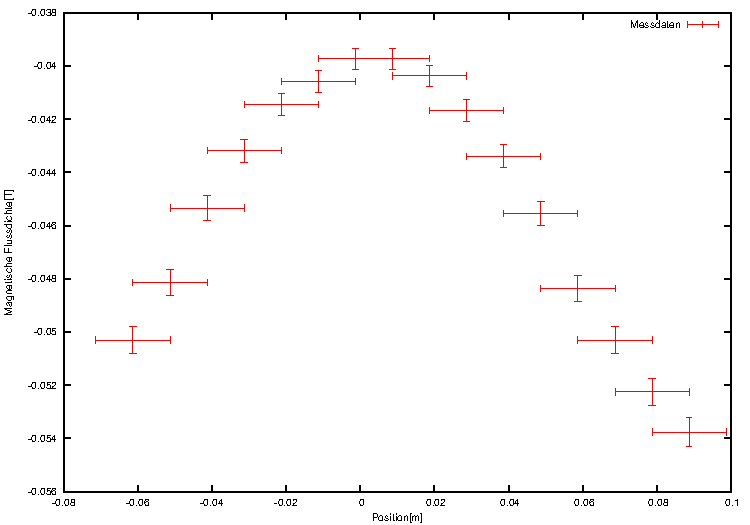
\includegraphics[scale = 1.3]{aufgabe_4.pdf}
  	\caption[Magnetfischerfluss in Abhängigkeit der Position]{Magnetfischerfluss in Abhängigkeit der Position}
  \label{fig:kasten}
\end{figure}

\newpage
\subsection{Aufgabe 5}
In der letzten Aufgabe sollte im ersten Teil der Innenwiderstand der Hallsonde bestimmt werden. Der Innenwiderstand wurde mit Formel \ref{eqn:innen_widerstand} und der Fehler mit Formel \ref{eqn:innen_widerstand_sigma} bestimmt. Es ergab sich ein Wert von 28,5 $(\pm 0,4)$ Ohm.

Zum Schluss sollte der Versatz $\Delta\text{x}$ der Hallspannungsabfriffe bestimmt werden, dafür wurde Formel \ref{eqn:delta} werwendet und für den Fehler wurde Formel \ref{eqn:delta_sigma} verwendet. Es ergab sich ein Wert von 0,0019 $(\pm 0,0002)$.


\section{Diskussion}

In Aufgabe 2 sollten wir die Spule an unser Netzgerät anschließen. Bei unserem Netzgerät war es nicht möglich einen Strom von einem Ampere einzustellen und wir mussten es mit einem anderen tauschen. Beim Anschließen des zweiten bzw. dritten Netzgerätes (wir haben insgesamt dreimal gewechselt, da das zweite Netzgerät keine Digitalanzeige hatte) haben wir nicht mehr auf die Polarität geachtet.\\
Danach haben wir die 12V Festpannungsquelle an unser Versuchskästchen angeschlossen und einen maximalen Hallstrom von 100mA eingestellt.\\
Zuletzt musste die Hallsonde in die Mitte der Spule geschoben werden.\\
In Aufabe 3 haben wir die optimale Position der Hallsonde am maximalen Ausschlag des Potentiometers eingestellt, das Magnetfeld nach Gleichung \ref{eqn:Aufgabe 3_TD_B-Feld_2} berechnet und mit dem gemessenen Wert nach Gleichung \ref{eqn:Aufgabe 3_TD_B-Feld_1} verglichen.\\
In der darauffolgenden Messung wurde der Spulenstrom variiert um die Abhängigkeit zwischen Hallspannung und Magnetfeld zu ermitteln. Dabei ist nicht sofort aufgefallen, dass das Potentiometer bei geringem Spulenstrom ein größeres Verhältnis von R$_2$ zu R$_1$ + R$_2$ anzeigte als bei 100mA Maximalstrom, was an der womöglich falschen Polung der Spule lag. Aus der negativen Steigung dieser Messung ergaben sich eine negative Hallkonstante und eine negative Teilchendichte, wie man an Plot \ref{fig:hall_mag}
unschwer erkennen kann.\\
Im letzten Teil der Aufgabe sollte der Zusammenhang zwischen Hallspannung und Hallstrom mit und ohne Magnetfeld ermittelt werden. Wie erwartet nahm die Hallspannung linear mit dem Hallstrom ab. Dabei fiel während der Messung nicht auf, dass die Verhältnisse von R$_2$ zu R$_1$ + R$_2$, die das Potentiometer ohne Magnetfeld anzeigte, größer waren als die Verhältnisse, die mit Magnetfeld angezeigt wurden.
 %Werte stimmen mit den Formeln überein/nicht überein

\end{document}

